\PassOptionsToPackage{subsection=false}{beamerouterthememiniframes}


\documentclass[usenames,dvipsnames,t]{beamer}


%
% Choose how your presentation looks.
%
% For more themes, color themes and font themes, see:
% http://deic.uab.es/~iblanes/beamer_gallery/index_by_theme.html
%
\mode<presentation>
{
  \usetheme{Antibes}      % or try Darmstadt, Madrid, Warsaw, ...
%  \usecolortheme{seahorse} % or try albatross, beaver, crane, ...
\usepackage{xcolor}  
\definecolor{nyuv}{RGB}{87,6,140}
%\definecolor{yblue}{RGB}{5.9,30.2,57.3}
\definecolor{yblue}{HTML}{00356b}
\usecolortheme[named=yblue]{structure}
 \usefonttheme[options]{serif}  % or try serif, structurebold, ...
  \setbeamertemplate{navigation symbols}{}
  \setbeamertemplate{caption}[numbered]
} 



\setbeamertemplate{headline}{}

\setbeamertemplate{footline}
{%
    \begin{beamercolorbox}[colsep=1.5pt]{upper separation line foot}
    \end{beamercolorbox}
    \begin{beamercolorbox}[ht=2.5ex,dp=1.125ex,%
        leftskip=.3cm,rightskip=.3cm plus1fil]{author in head/foot}%
        \leavevmode{\usebeamerfont{author in head/foot}\insertshortauthor}%
        \hfill%
        \leavevmode{\usebeamerfont{title in head/foot}\insertshorttitle}%
        \hfill%
        {\usebeamerfont{institute in head/foot}\usebeamercolor[fg]{institute in head/foot}
%        {\sc\insertframenumber}
%        {\hyperlink{appxhome}{\beamerbutton{\tiny$\cdot$}}}
        {\hyperlink{appxhome}{\insertframenumber}}
        }%
    \end{beamercolorbox}%
    \begin{beamercolorbox}[colsep=1.5pt]{lower separation line foot}
    \end{beamercolorbox}
}

\setbeamersize{text margin left=7mm,text margin right=7mm} 
\setbeamercolor{button}{bg=nyuv,fg=white}
\newcommand{\beamerbuttontwo}[1]{%
    \begingroup% keep color changes local
    \setbeamercolor{button}{fg=black,bg=lightgray}%
    \beamerbutton{#1}% original definition
    \endgroup
    }

\setbeamertemplate{itemize items}[circle]


\usepackage{dcolumn}
\usepackage{multirow}

\usepackage{soul}


%\usepackage{enumitem}

%\newcommand{\inlineitem}{%
%\leavevmode\usebeamertemplate{itemize item}
%}
%\newcounter{newenumi}
%\setcounter{newenumi}{1}
%
%\newcommand{\inlineenum}{%
% {%
% \setcounter{enumi}{\thenewenumi}%
% \leavevmode\usebeamertemplate{enumerate  item}
% \stepcounter{newenumi}
% \setcounter{enumi}{0}
% }
%}
%
%\newcommand{\resetinlineenum}{
% \setcounter{newenumi}{1}
%}



\usepackage{graphicx}
%\graphicspath{{../HM-images/presentationeshwari}}

\usepackage{caption}
\usepackage{subcaption}

\usepackage[english]{babel}
\usepackage[utf8x]{inputenc}

\usepackage[T1]{fontenc}

\usepackage{tcolorbox}
\newcommand\boxwhite[1]{\tcolorbox[arc=0pt,colback=white,size=fbox,colframe=white]\invisible<0| handout:1->{#1}\endtcolorbox}
\newcommand\boxblack[1]{\tcolorbox[width=35mm,arc=0pt,colback=white,size=fbox,colframe=nyuv]\invisible<0| handout:1->{#1}\endtcolorbox}

\newcommand\Wider[2][3em]{%
\makebox[\linewidth][c]{%
  \begin{minipage}{\dimexpr\textwidth+#1\relax}
  \raggedright#2
  \end{minipage}%
  }%
}

\usepackage{array}


\usepackage{ragged2e}
\usepackage{changepage} % adjust margins of specific pages

\usepackage{tabularx}
\usepackage{tabu}
\usepackage{booktabs}
\usepackage{makecell}
\setcellgapes{4pt} %parameter for the spacing

\usepackage[export]{adjustbox}


\usepackage{minibox}


\usepackage{animate}




\newcommand{\RM}[1]{{\color{red} [RM]: #1}}

\newcommand{\outgr}{outgroup }
\newcommand{\outgrp}{outgroup}


\newcommand*{\TextVCenter}[1]{%
  \text{$\vcenter{\hbox{#1}}$}%
}
\newcommand{\shsqr}{\TextVCenter{{\tiny $\blacksquare$}}}


\title[]{{ 
\large \bf Reducing WhatsApp Usage to Mitigate Misinformation Exposure During Elections: Evidence from a Multi-Country Experiment}
% \\  \line(1,0){300}
}
\author[]{\small Rajeshwari Majumdar \\ Tiago Ventura \\ Shelley Liu \\ Carolina Torreblanca \\ Joshua A. Tucker}
\date{\footnotesize %  location \\ 
\vspace{.25cm} 

APSA Annual Meeting \\
September 6, 2024
}



%\AtBeginSection[]
%{
%    \begin{frame}
%        \frametitle{Table of Contents}
%        \tableofcontents[currentsection]
%    \end{frame}
%}

\begin{document}

\begin{frame}[plain]
  \titlepage
\end{frame}

% Uncomment these lines for an automatically generated outline.
%\begin{frame}{Outline}
%  \tableofcontents
%\end{frame}



\section{Introduction}



\begin{frame}{Motivation} \small  

\vspace{.25cm} 
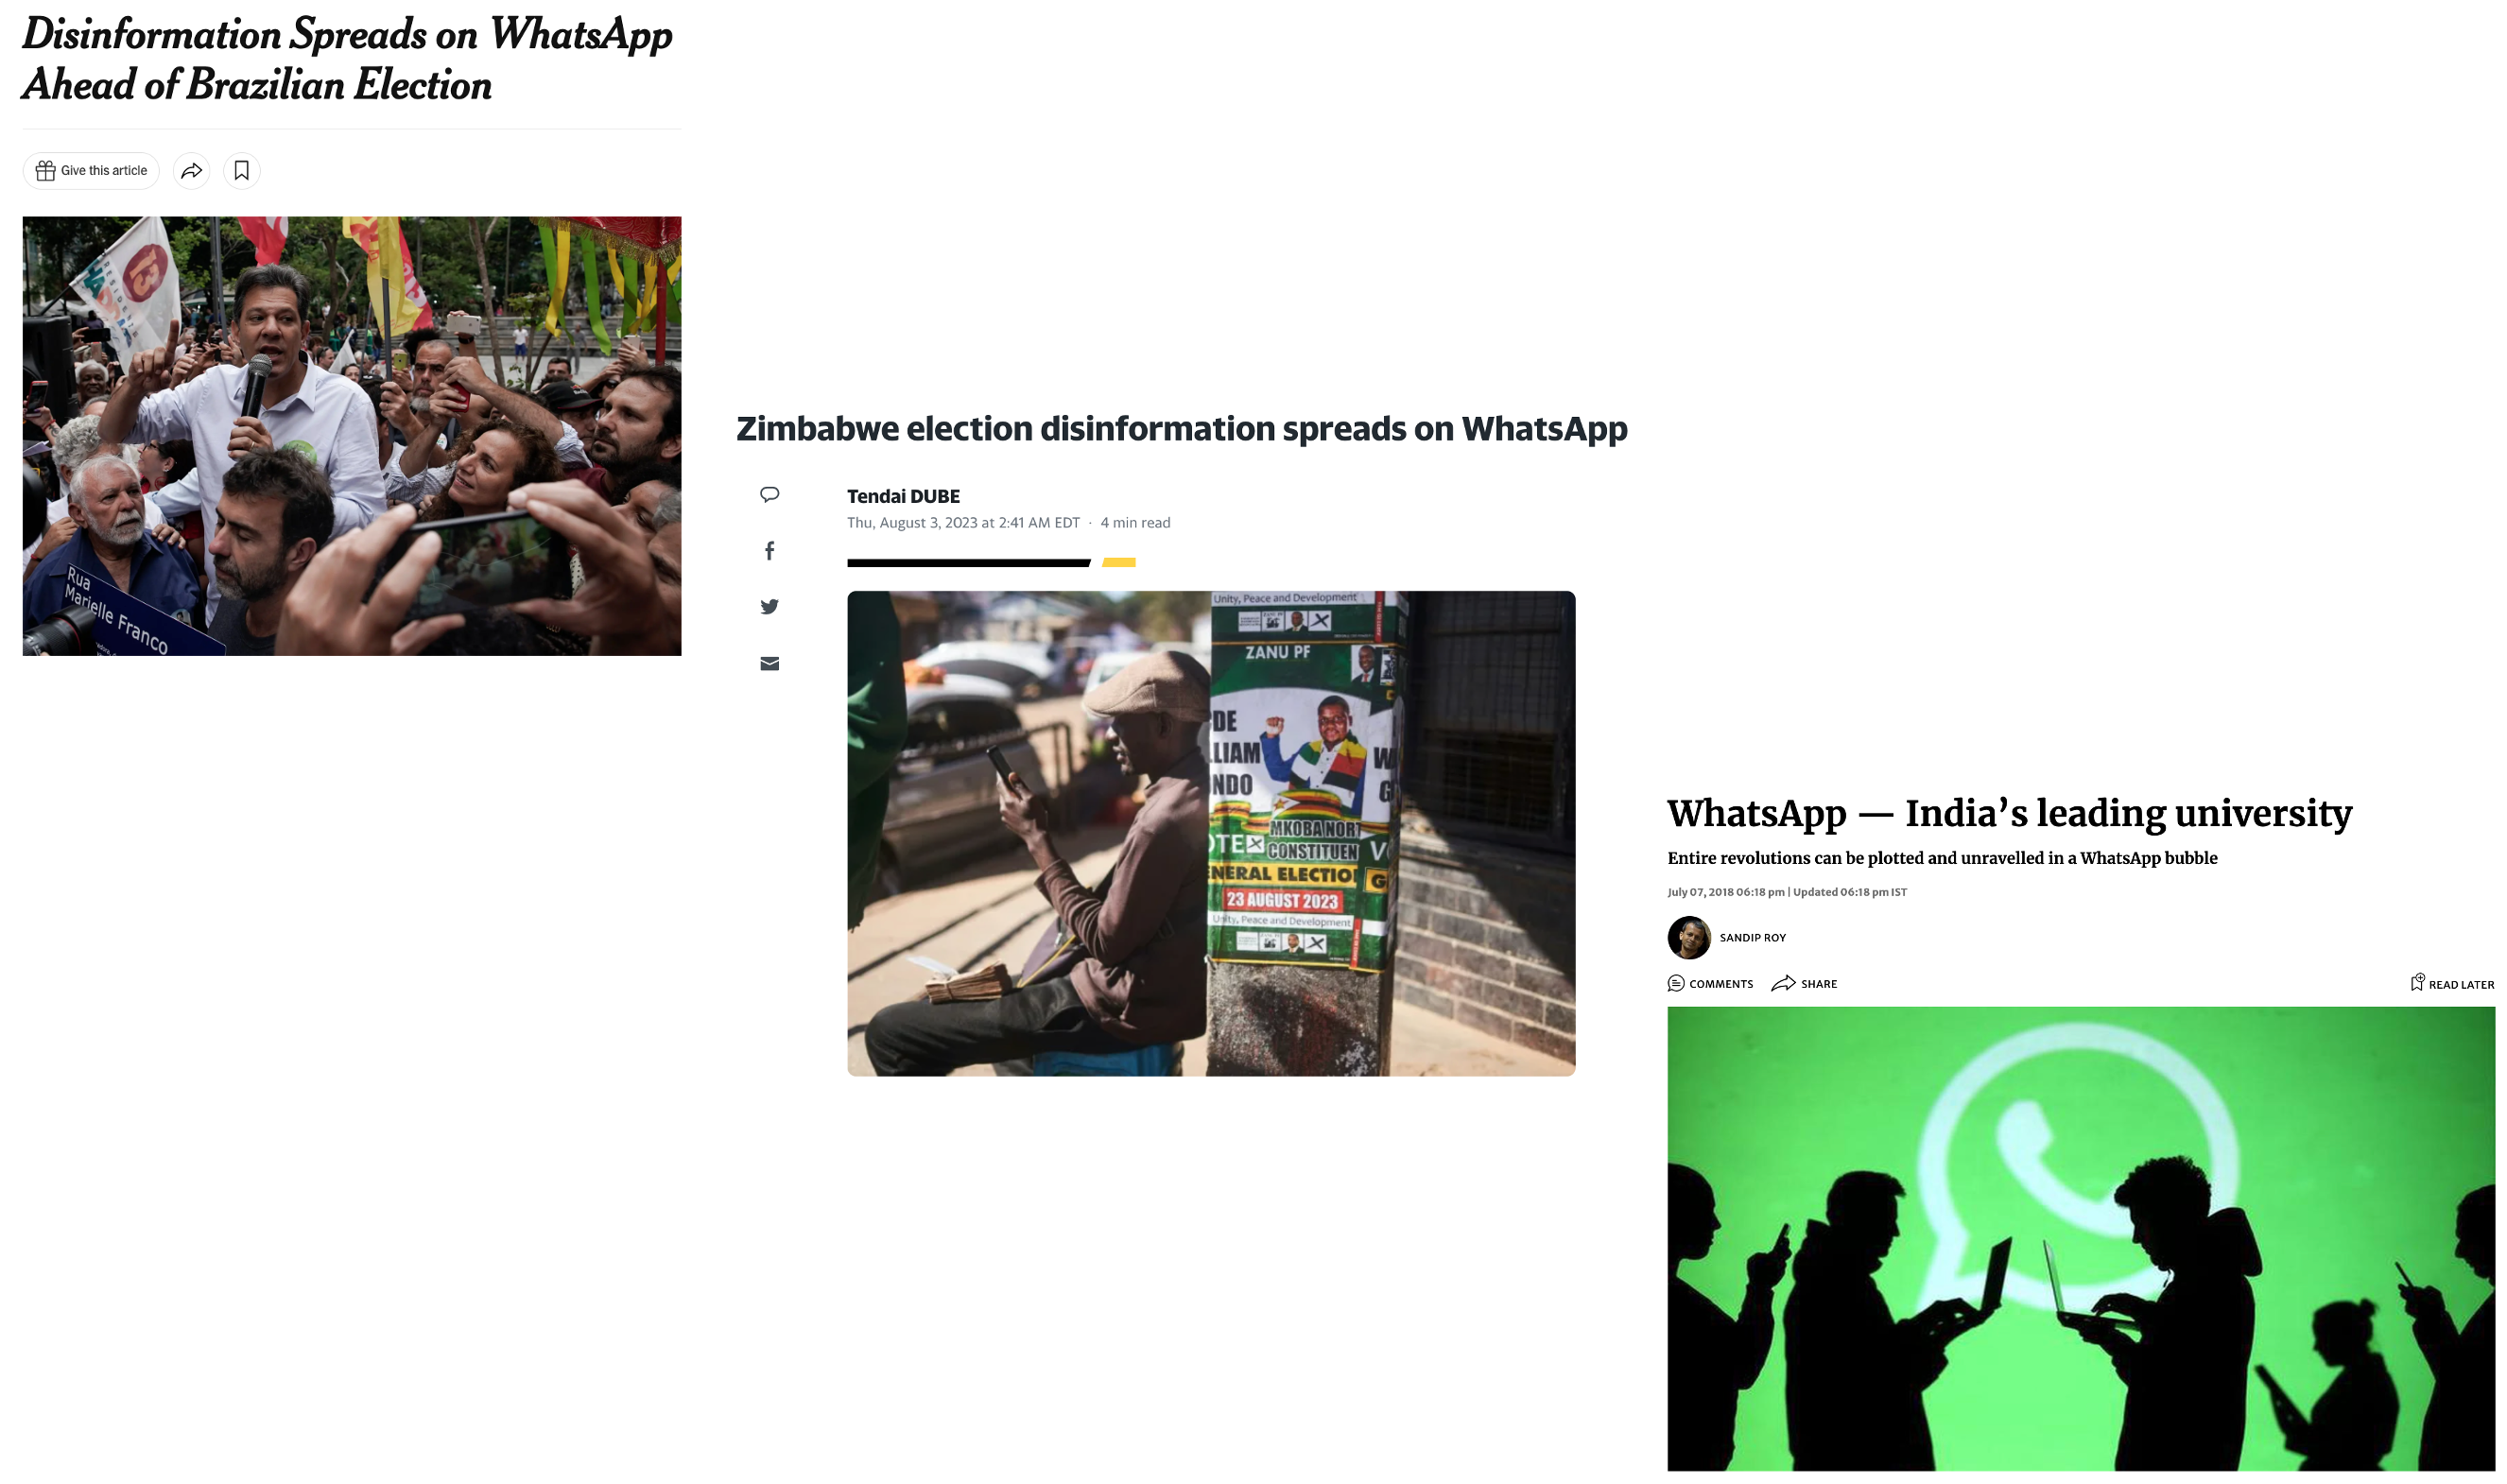
\includegraphics[scale=.25]{whatsappmotivation}

\end{frame}


\begin{frame}{Research on Social Media and Misinformation} \small  

\vspace*{\fill}

\begin{itemize}
\item Existing research: focused primarily on feed-based platforms that are popular in advanced democracies (Twitter, Facebook) %\pause
\item But in the Global South %\pause
	\begin{itemize}
	\item the types of social media platforms that are predominantly used are fundamentally different (message-based; WhatsApp)\vspace{.1cm}%\pause
	\item the harmful offline consequences of misinformation exposure may be more pronounced
	\end{itemize}
\end{itemize}

\vspace*{\fill}

\end{frame}


\begin{frame}{Our Goal} \small  

\vspace*{\fill}

\centering
Identify the causal effects of WhatsApp usage on exposure to misinformation and downstream effects on users’ political attitudes 

\vspace*{\fill}

\end{frame}


\begin{frame}{Approach} \small  

\vspace*{\fill}

\centering
WhatsApp ``deactivation'' experiment in India and South Africa during the month leading up to their most recent general elections

\vspace*{\fill}

\end{frame}


\begin{frame}{Classical Deactivation Studies} \small  

\vspace*{\fill}

\centering
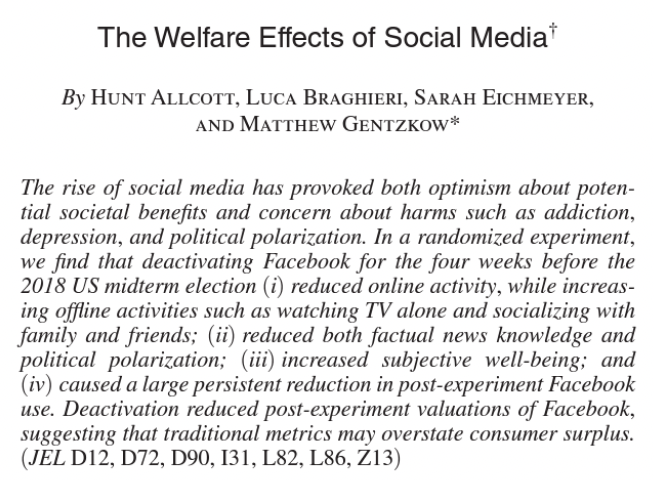
\includegraphics[scale=.2]{deactivation_studies_allcott} \hspace{.25cm}
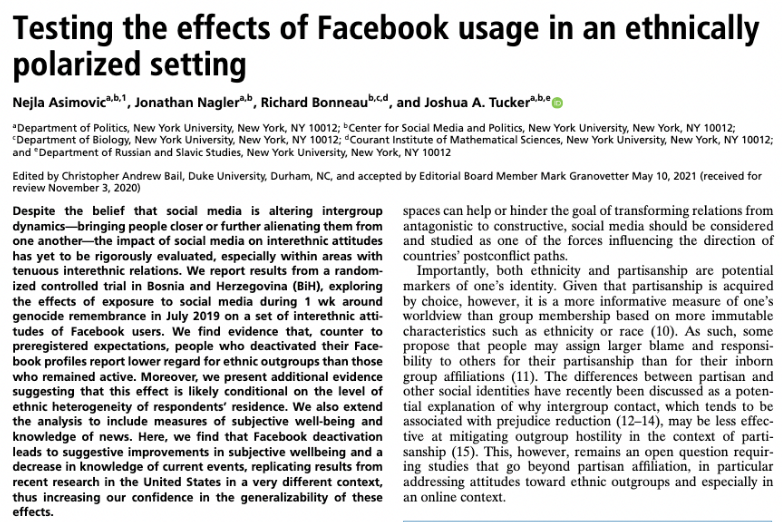
\includegraphics[scale=.2]{deactivation_studies_asimovic}

\vspace*{\fill}

\end{frame}




\begin{frame}{This Study} \small  

\vspace*{\fill}

\begin{itemize}
\item \textbf{Problem:} Fully deactivating WhatsApp is neither possible nor ideal \pause

\item \textbf{Our proposed workarounds:}

\begin{enumerate}
\item Impose a time limit on WhatsApp usage  \vspace{.1cm} % \pause
\item Cut the primary channels through which users are exposed to misinformation and polarizing content: videos, images \& audio \pause
\end{enumerate}

\item \textbf{Modified deactivation experiment:} 
\begin{enumerate}
\item Incentivize participants to either limit their daily WhatsApp usage or refrain from looking at multimedia content\vspace{.1cm} \pause
\item Test whether these restrictions reduce exposure to election (mis)information\vspace{.1cm} \pause
\item Test whether reduced exposure leads to changes in political attitudes 
\end{enumerate}

\end{itemize}

\vspace*{\fill}

\end{frame}



\begin{frame}{Hypotheses} \small  

Compared to those who use WhatsApp without any restrictions, those who are randomly assigned to reduce WhatsApp usage will:	\pause

\vspace{.2cm}

\begin{itemize}
\item given changes in consumption habits, 
\end{itemize}
\vspace{-.2cm}
\begin{itemize}\setlength{\itemindent}{2em} \small
\item[H1a:] \color{yblue}  report lower levels of exposure to false information
\item[H1b:] \color{yblue}  report lower levels of exposure to true information
\end{itemize}	\pause

\begin{itemize}
\item considering theories of repeated exposure on accuracy perceptions, 
\end{itemize}
\vspace{-.2cm}
\begin{itemize}\setlength{\itemindent}{2em} \small
\item[H2a:] \color{yblue}  be more likely to accurately identify false information as false
\item[H2b:] \color{yblue}  be less likely to accurately identify true information as true
\end{itemize}	\pause

\begin{itemize}
\item given likely reduction in exposure to misinformation and hate speech,
\end{itemize}
\vspace{-.2cm}
\begin{itemize}\setlength{\itemindent}{2em} \small
\item[H3a:] \color{yblue}    exhibit lower levels of partisan polarization
\item[H3b:] \color{yblue}    exhibit lower levels of ethnic/racial prejudice
\end{itemize}



 


\end{frame}


\section{Experimental Design}


\begin{frame}[plain]
\vspace{3cm}
\centering
\LARGE 
Experimental Design
\end{frame}

\begin{frame}{Experimental Conditions} \small  

{\bf \color{yblue} Types of partial deactivation}
\begin{itemize}
\item Time: Limit daily WhatsApp usage to 10 minutes 
\item Media: Do not consume multimedia content received via WhatsApp
\end{itemize}

\vspace{.5cm}\pause


{\bf \color{yblue} Treatment and control}
\begin{itemize}
\item Treatment: Change {settings \textit{and} behavior} for \textbf{4 weeks} (one month) leading up to election
\item Control: Change only {behavior} for \textbf{3 days} a month before election
\end{itemize}

\vspace{.5cm}\pause


{\bf \color{yblue} $\rightarrow$ 2 $\times$ 2 design}

\begin{table}[]
\begin{tabular}{|c|c|}
\hline Time Treatment & Time Control \\ \hline Media Treatment & Media Control \\ \hline
\end{tabular}
\end{table}


\end{frame}



\begin{frame}{Treatment 1: Time Reduction} \small %  \pause
\vspace{-.2cm}

{\color{yblue} \bf Task}
\begin{itemize}
\onslide<1->{\item Treatment: For 4 weeks, limit daily usage to 10 minutes per day\\  \hspace{1.75cm} and set a daily app timer of 10 minutes}
\only<1>{\item Control: For 3 days, limit daily usage to 10 minutes}
\end{itemize}


\only<2>{
{\color{yblue} \bf Checking compliance} 

\vspace{.1cm}

\centering\fbox{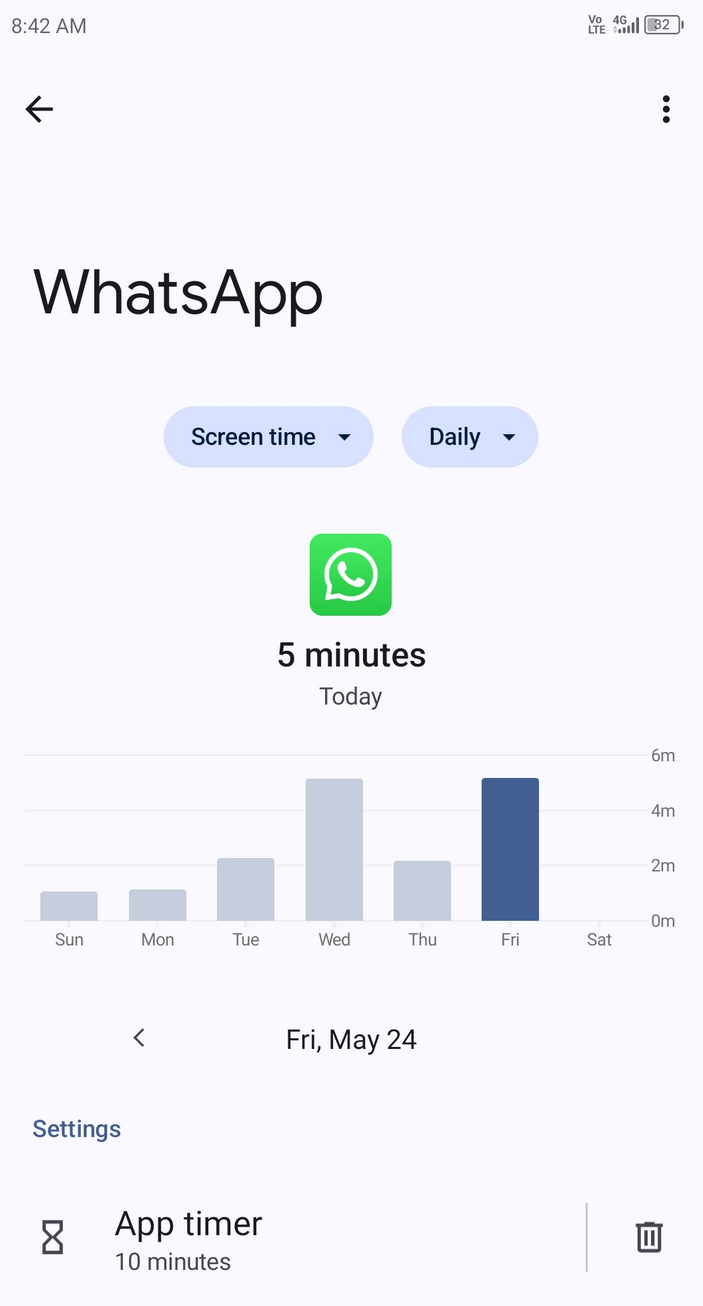
\includegraphics[scale=.12]{ss_ttime_actualsubject_lightmode}}
}


\end{frame}




\begin{frame}{Treatment 2: Multimedia Deactivation} \small  
\vspace{-.2cm}

{\color{yblue} \bf Task}
\begin{itemize}
\onslide<1->{\item Treatment: For 4 weeks, do not consume multimedia \\  \hspace{1.75cm} and turn off the automatic download of multimedia}
\only<1>{\item Control: For 3 days, do not consume multimedia}
\end{itemize}

\onslide<2-4>{
{\color{yblue} \bf Automatic downloads}

\vspace{.1cm}
}

\only<2>{
\centering\fbox{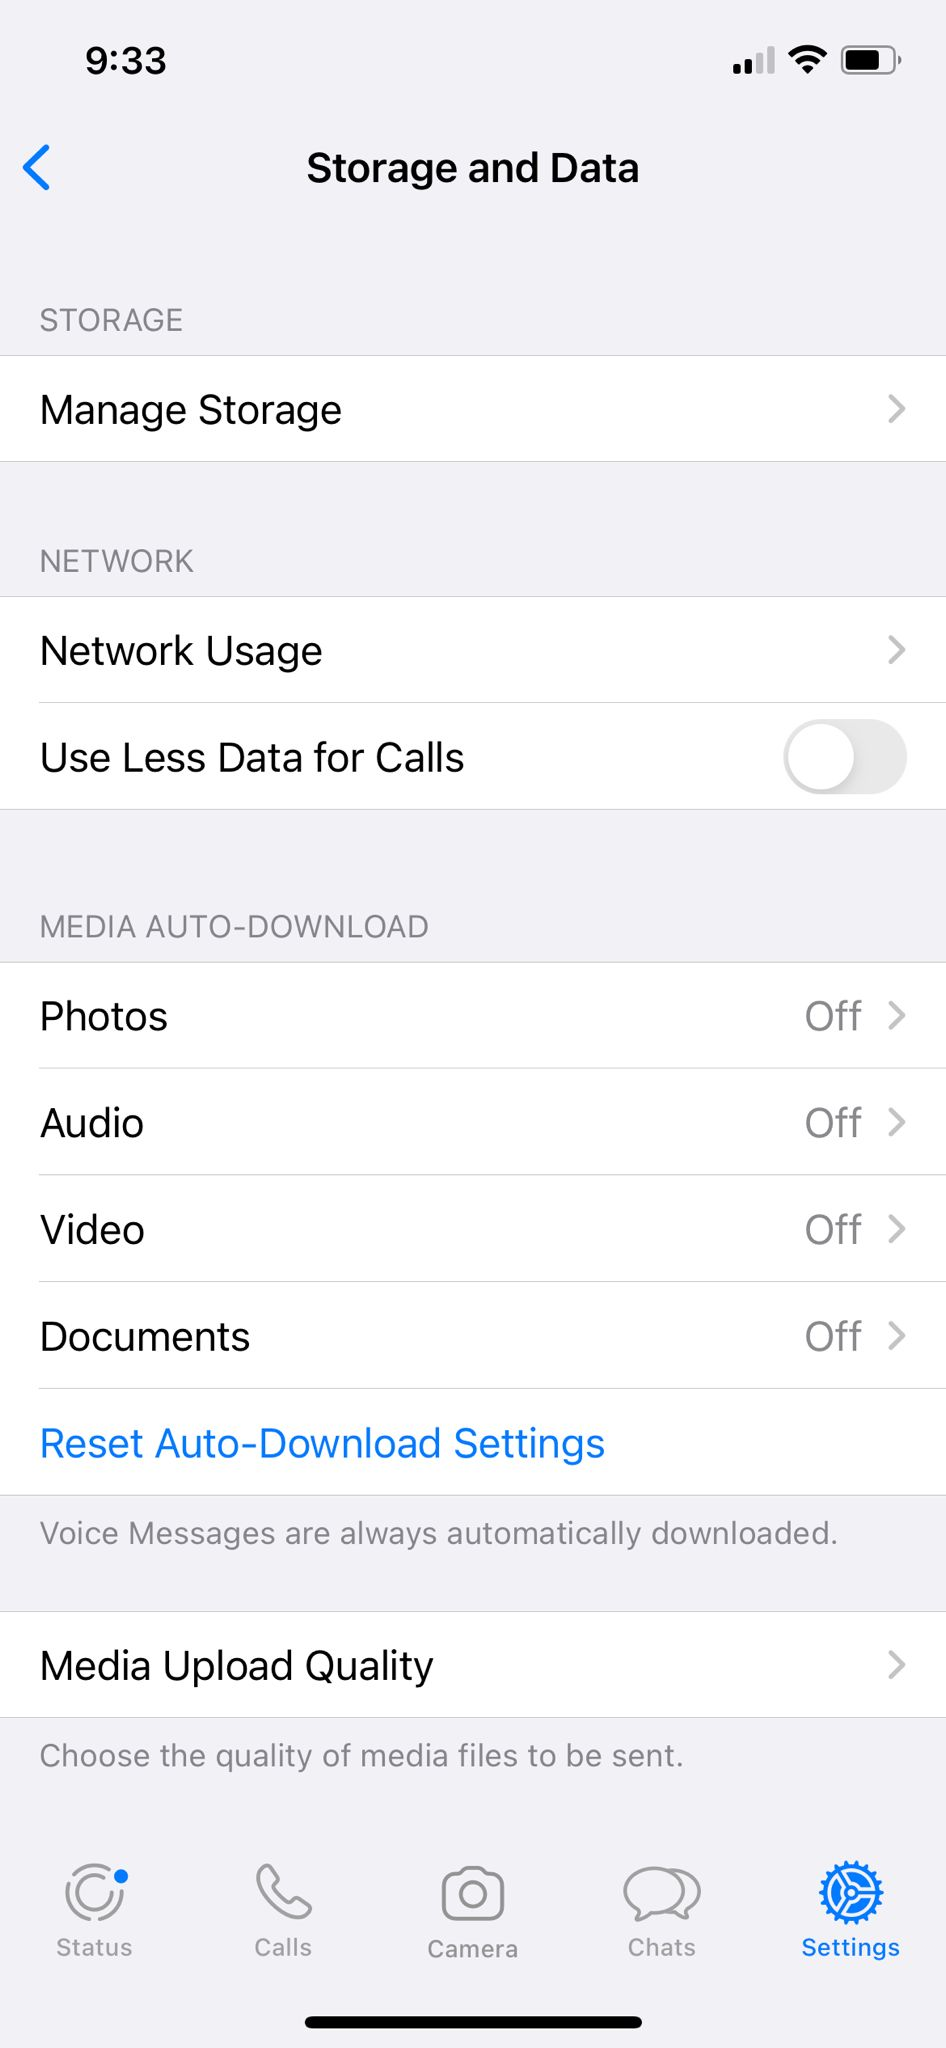
\includegraphics[scale=.08]{ss_tmedia_autodloff}}
}
\only<3>{
\centering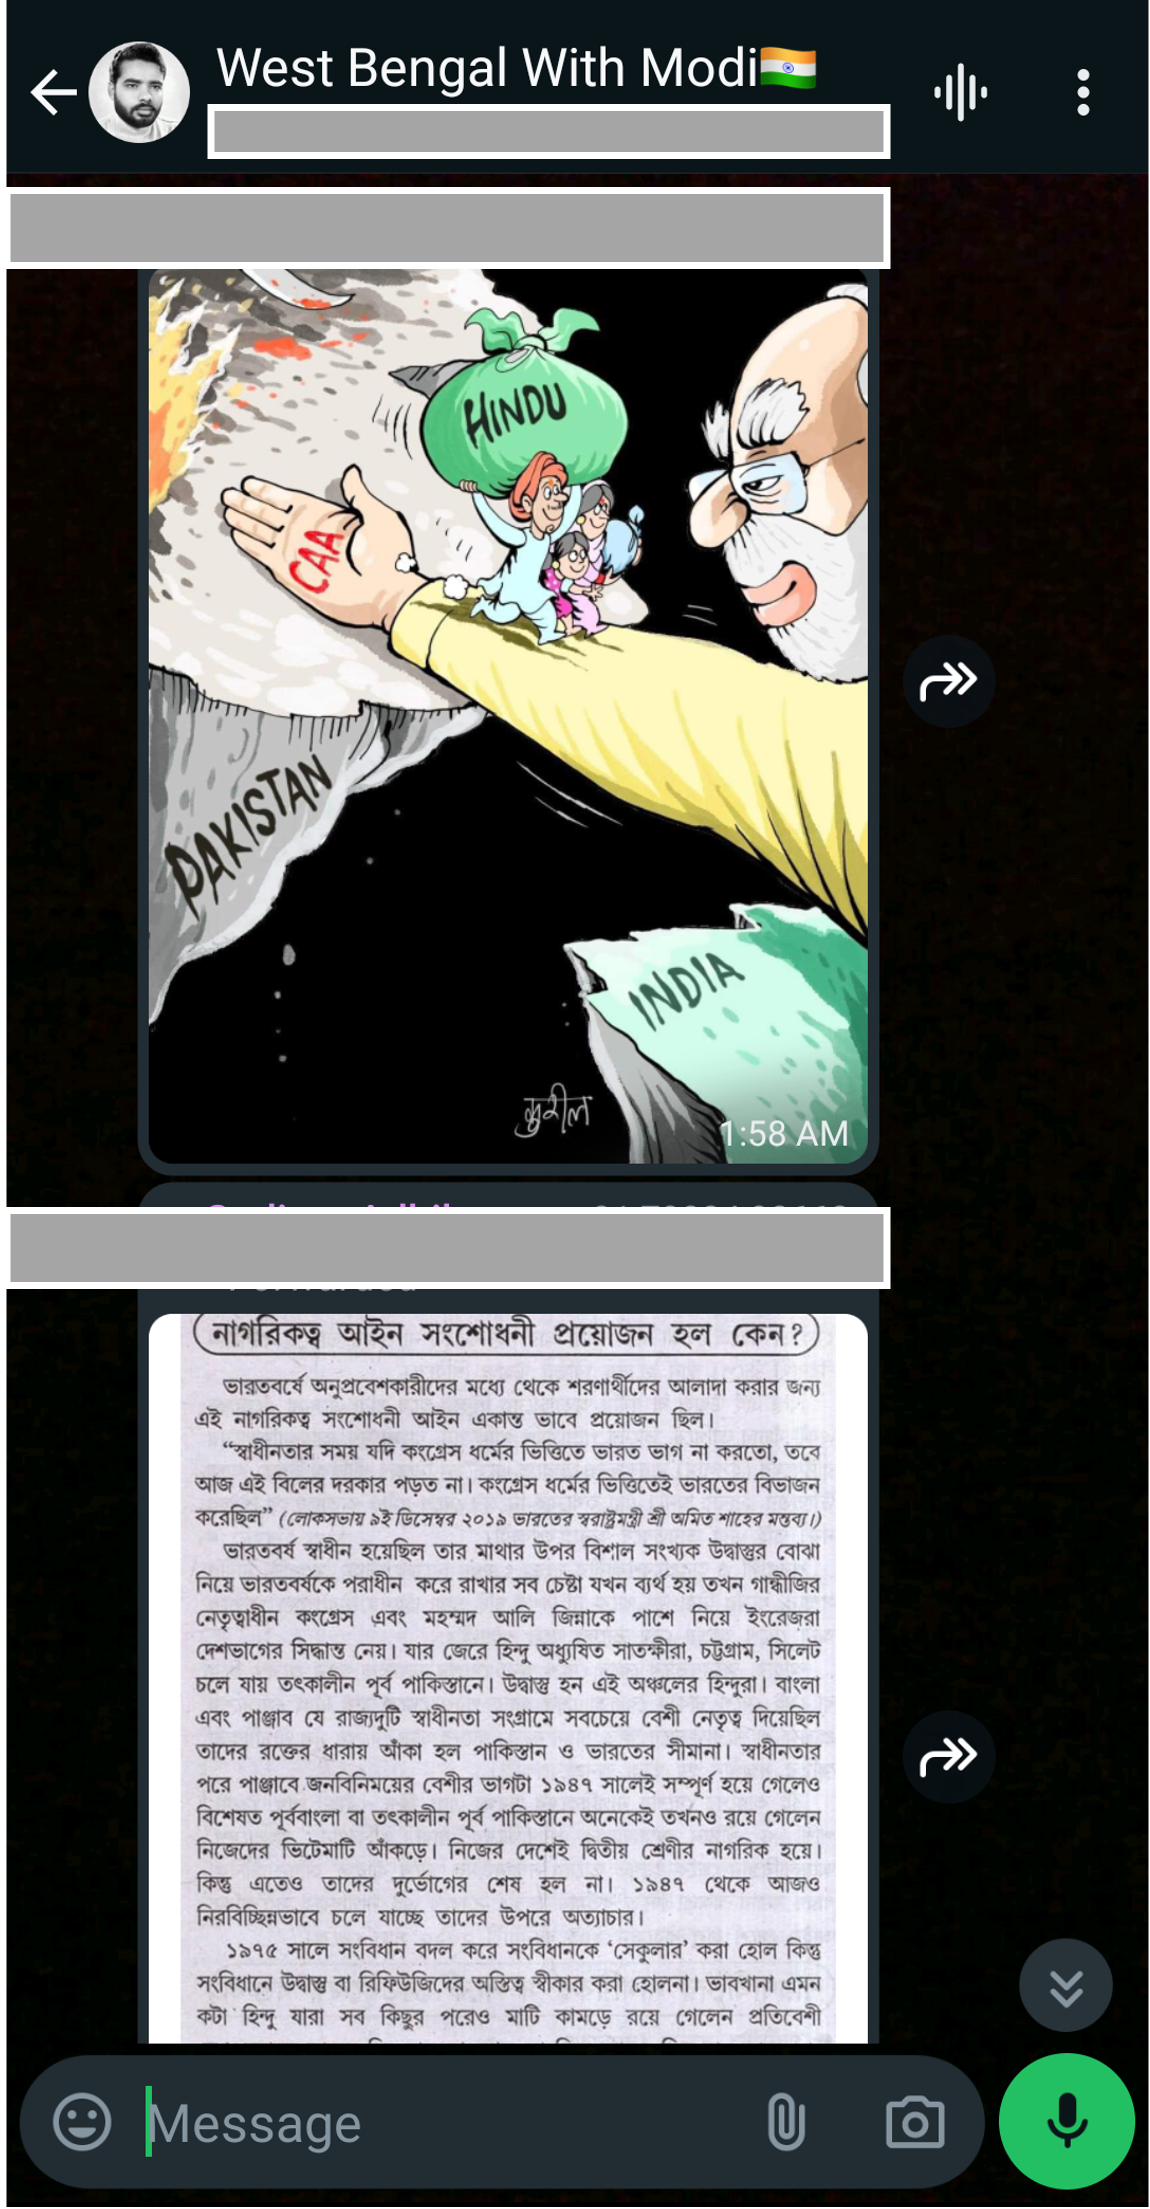
\includegraphics[scale=.35]{ss_tmedia_examplereal_dlpost}
}
\only<4>{
\centering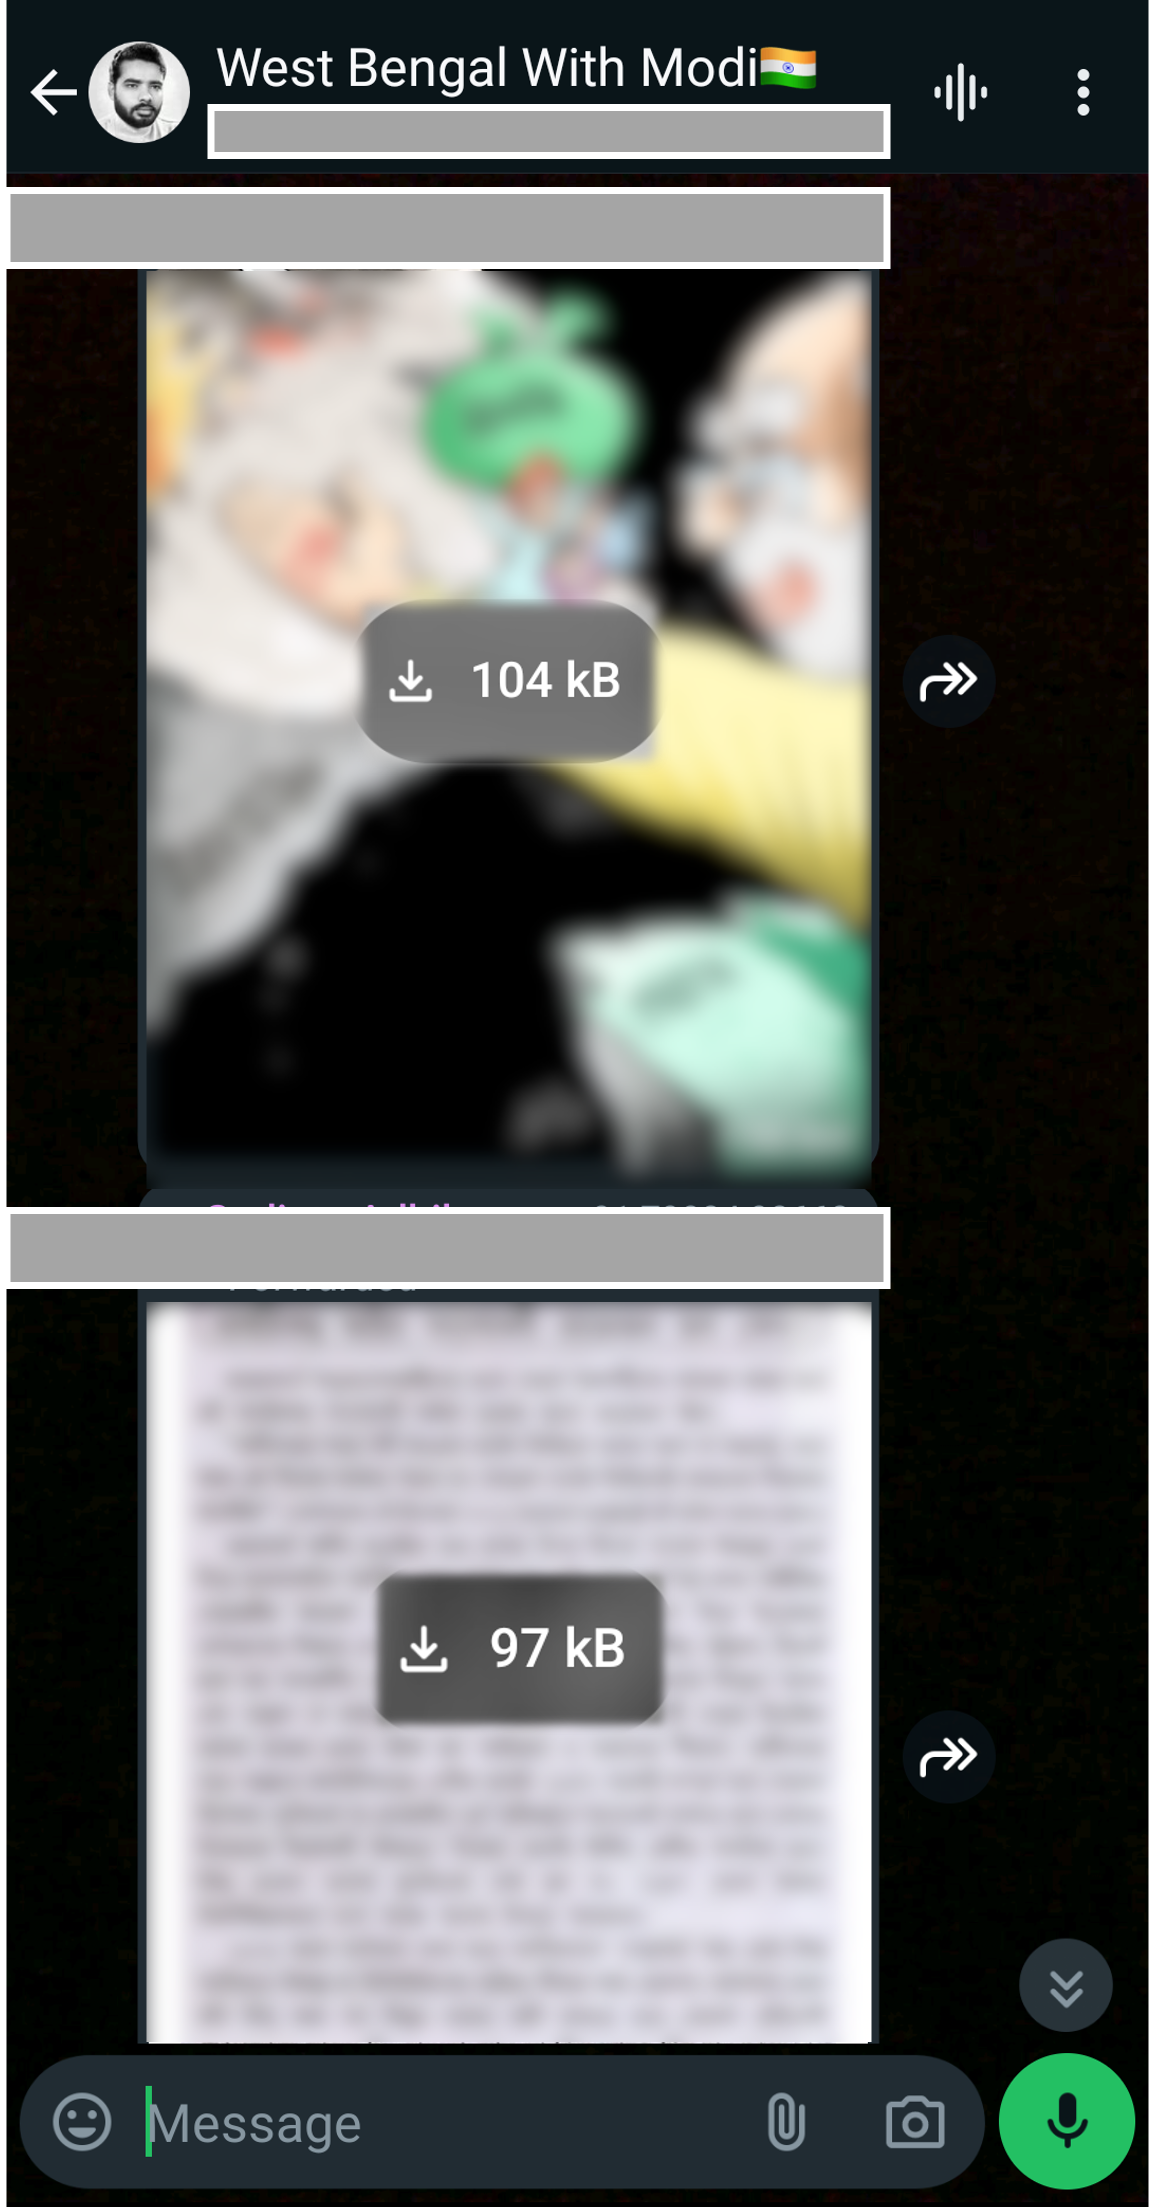
\includegraphics[scale=.35]{ss_tmedia_examplereal_dlpre}
}


\onslide<5->{
\vspace{-.55cm}

{\color{yblue} \bf Checking compliance}

\vspace{.1cm}
}

\onslide<5->{
\centering\fbox{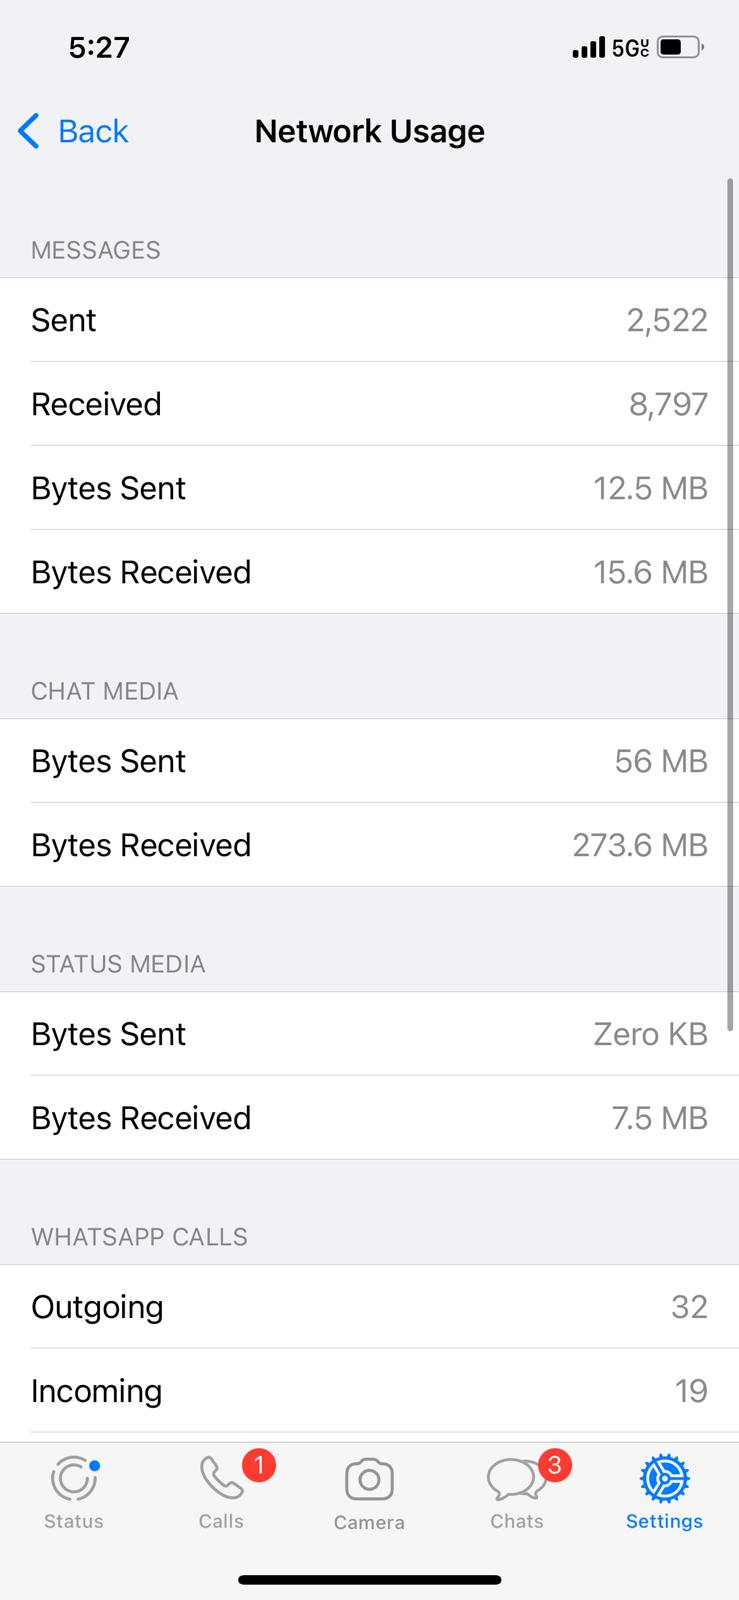
\includegraphics[scale=0.10]{ss_tmedia_networkusage}}
}



\end{frame}


\begin{frame}{Implementation} \small  
\vspace{-.25cm}

\begin{itemize}
\item Used Meta Advertisements to recruit WhatsApp users in India and South Africa% \pause
\item All participants could earn a total of \$15 for completing surveys and uploading weekly screenshots%\pause
\item Participants in treatment conditions who successfully reduced usage or multimedia consumption received an additional \$45 \pause
\item Timeline: 
\end{itemize}
\centering
\Wider[4em]{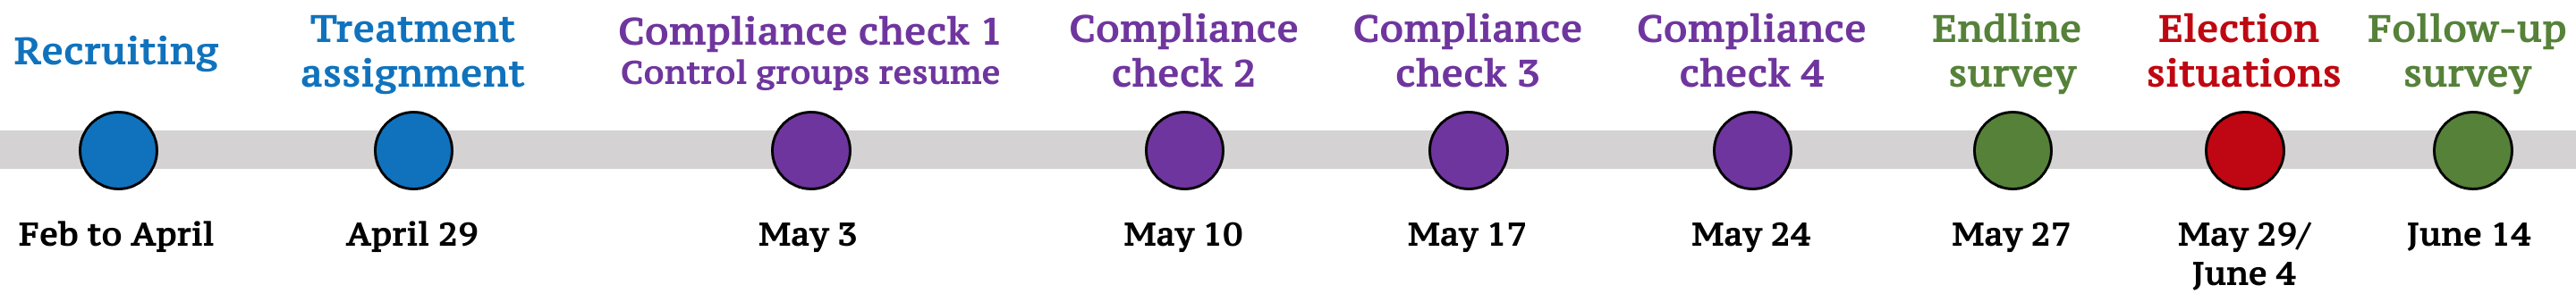
\includegraphics[scale=.252]{timelinefigure}}
\pause\vspace{-.15cm}
\begin{itemize}
\item Started with 1,498 respondents across the two countries;  1,394 (93\%) completed the endline survey 
\begin{table}\centering
\begin{tabular}{ccc}
\hline  
& Treatment & Control \\  \hline
Time & 91\% & 94\% \\
Media & 93\%  & 94\% \\
\hline
\end{tabular}
\end{table}
\end{itemize}

\end{frame}



%\begin{frame}{Compliance scene} \small  
%
%{\color{yblue} \bf Defining compliance in the Time condition}
%\begin{itemize}
%\item Submit weekly screenshots showing WhatsApp Screen Time
%\item Achieve modal daily usage of <10m in at least 2 of 4 weeks
%\item Do not exceed modal daily usage >30m during any week 
%\end{itemize}
%
%\vspace{.25cm}
%
%$\rightarrow$ 47\% of treated respondents complied 
%
%\vspace{.5cm} \hrule \vspace{.5cm}
%
%{\color{yblue} \bf Defining compliance in the Media condition}
%\begin{itemize}
%\item Submit weekly screenshots showing WhatsApp Storage Statistics
%\item Have a difference in bytes consumed that is smaller than the median difference among the control group
%\item Do not reset statistics during the experimental period 
%\end{itemize}
%
%\vspace{.25cm}
%
%$\rightarrow$ 53\% of treated respondents complied
%
%\end{frame}




\section{Results}


\begin{frame}[plain]
\vspace{3cm}
\centering
\LARGE 
Results
\end{frame}

%\begin{frame}{Overview} \small  
%
%List out outcomes 
%
%\end{frame}

\begin{frame}{Exposure to and Belief in News Headlines} \small  

\vspace*{\fill}

\begin{itemize}
\item 	Participants are shown 8 news headlines; asked (a) whether they have seen this news before \& (b) whether they think the news is true \pause
\item 	Four headlines are true news; four are misinformation stories \pause
\item		Count how many (a) recalled \& (b) accurately identified as T/F  \pause
\item		Means (sd) across the control conditions:  
\begin{table}\centering
\begin{tabular}{ccc}
\hline  
& True headlines & False headlines  \\  \hline
Prior exposure & 2.13 (1.30)  & 1.25 (1.18) \\
Think it is true &  2.39  (1.18) &  1.28  (1.15) \\
\hline
\end{tabular}
\end{table} 
\end{itemize} 

\vspace*{\fill}

\end{frame}



\begin{frame}{Exposure} \small  
Limiting WhatsApp usage reduces exposure to misinformation \& news
%DV: number of stories seen before (0-4)
\begin{center}
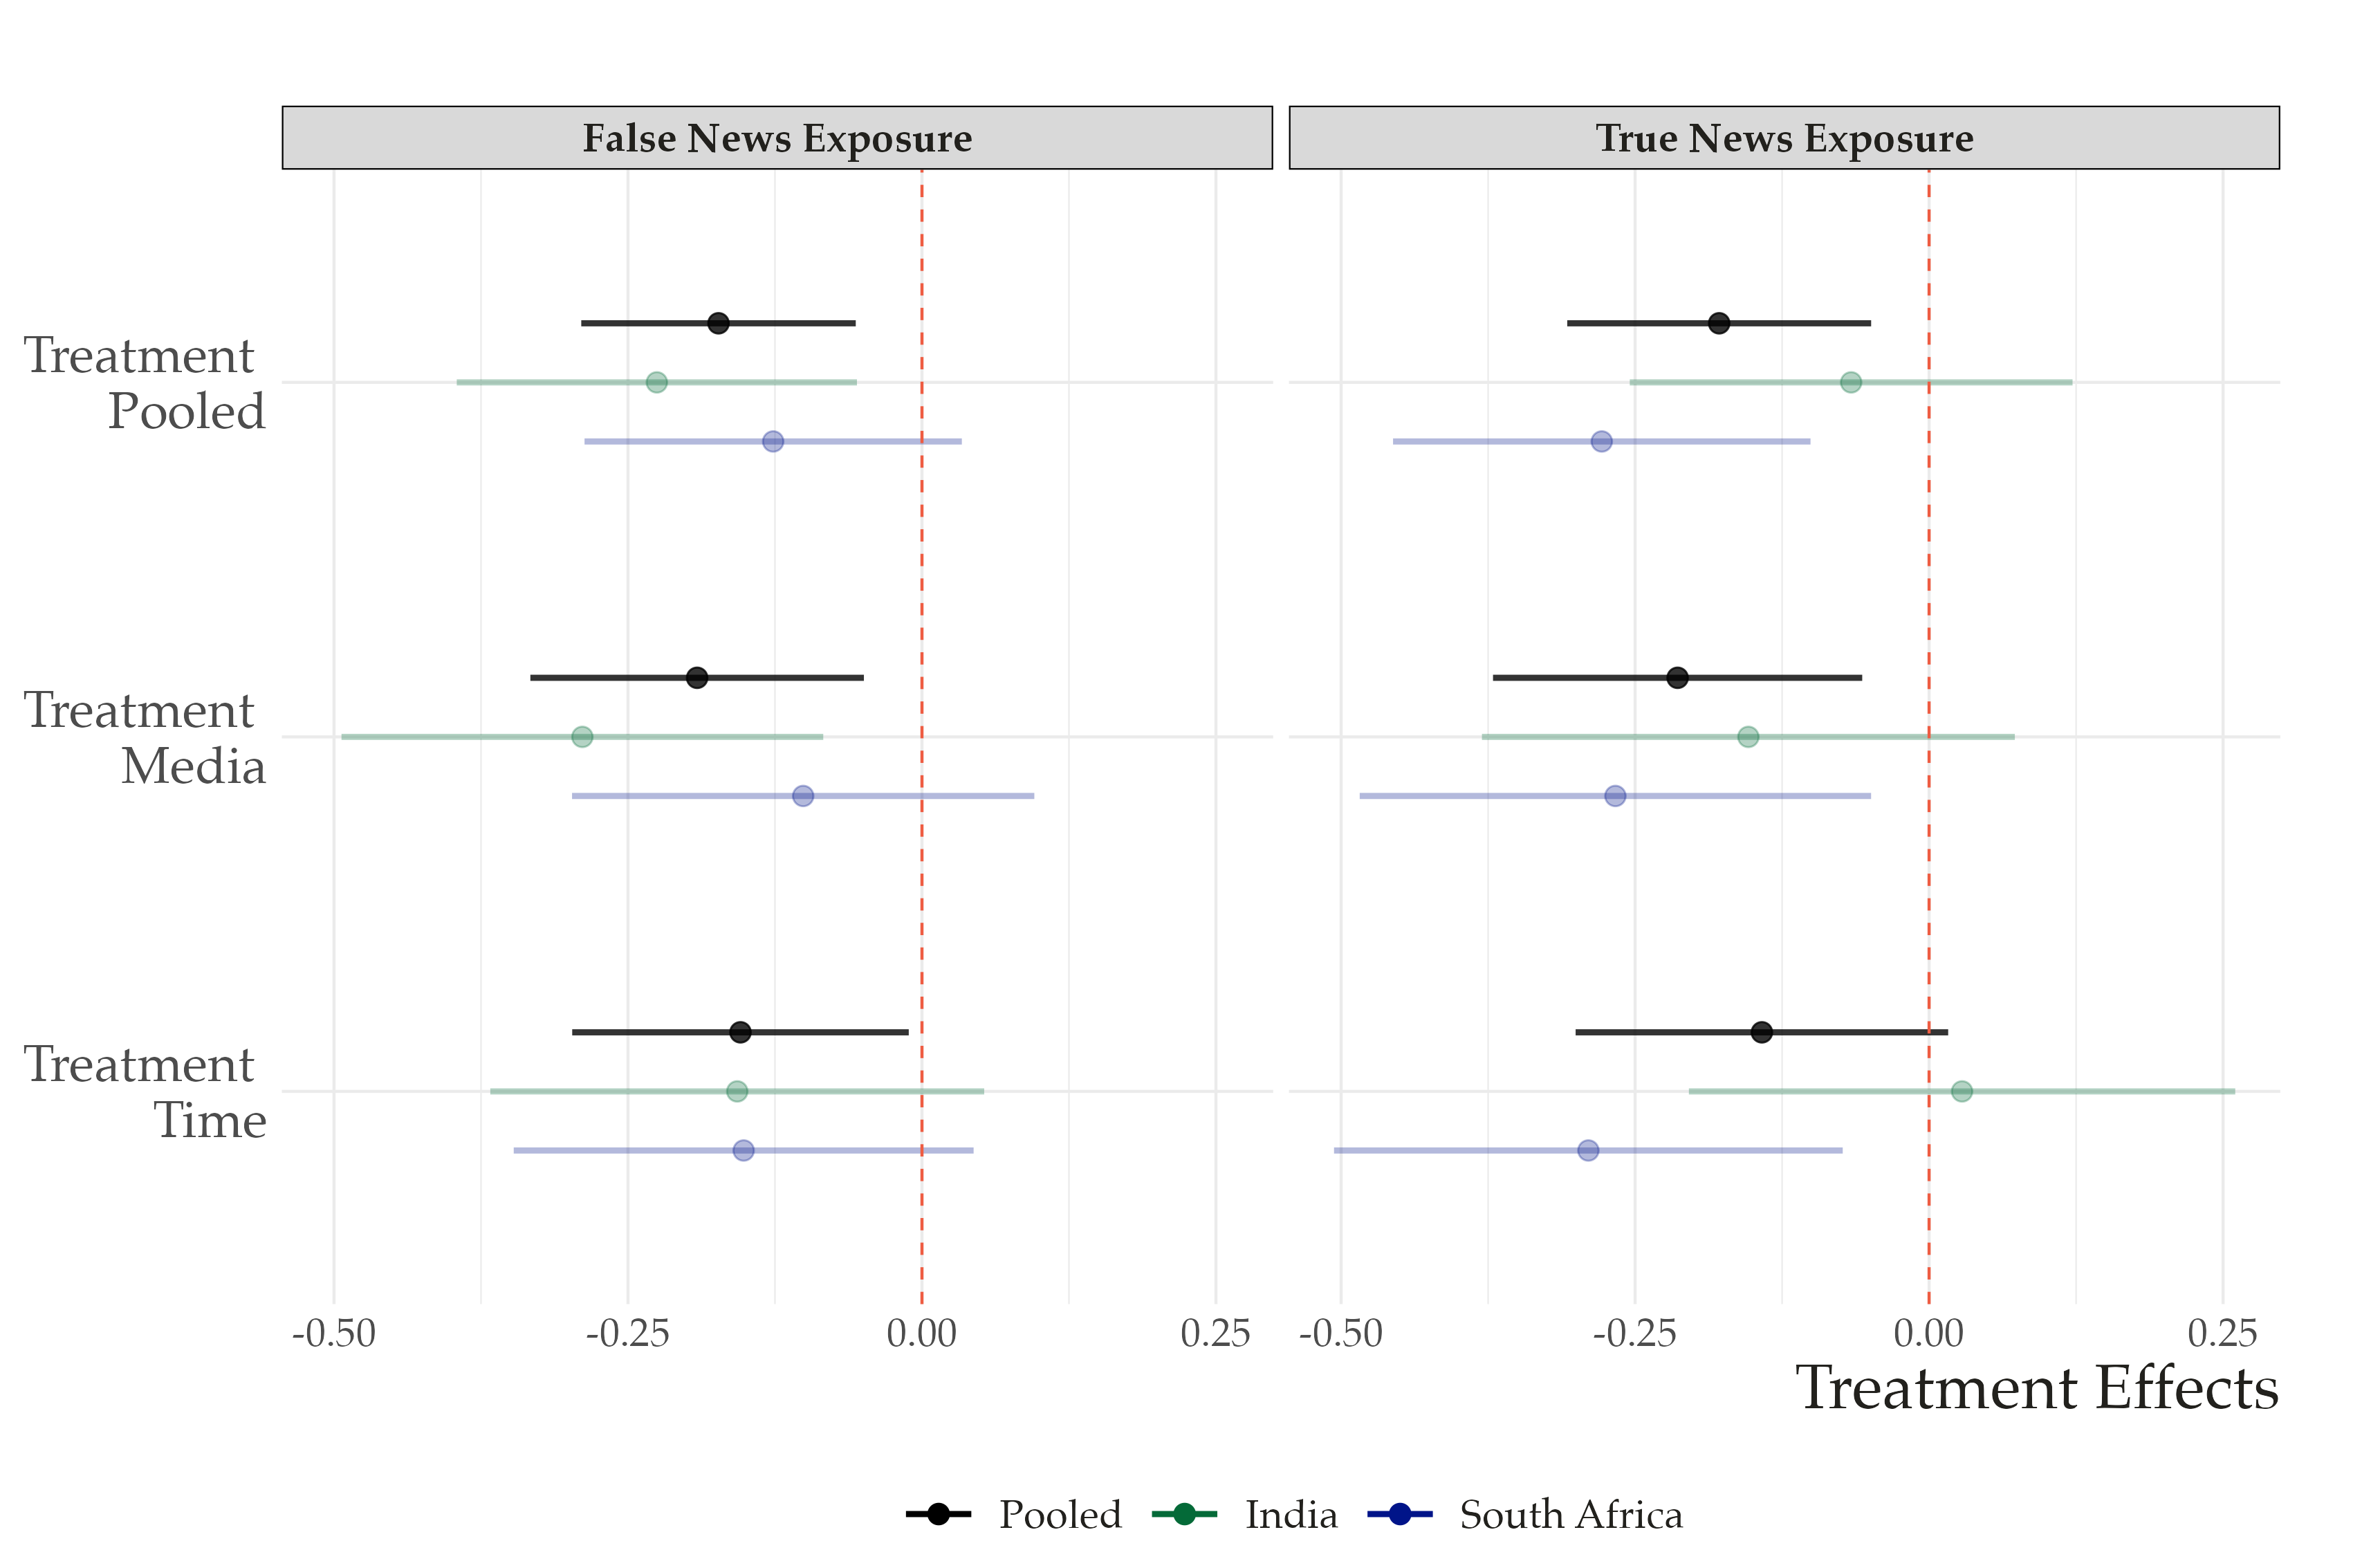
\includegraphics[scale=.37]{h1_itt}
\end{center}

%maybe say broad takeaway: slightly stronger results for misinfo in india but true news in SA; in India pro-BJP misinfo less recalled, SA no clear pattern on political alignment 

\end{frame}


\begin{frame}{Belief} \small  
A short-term reduction in exposure does not translate to changes in accuracy judgments
%DV: number of stories believed to be true (0-4)
%\vspace{-.25cm}
\begin{center}
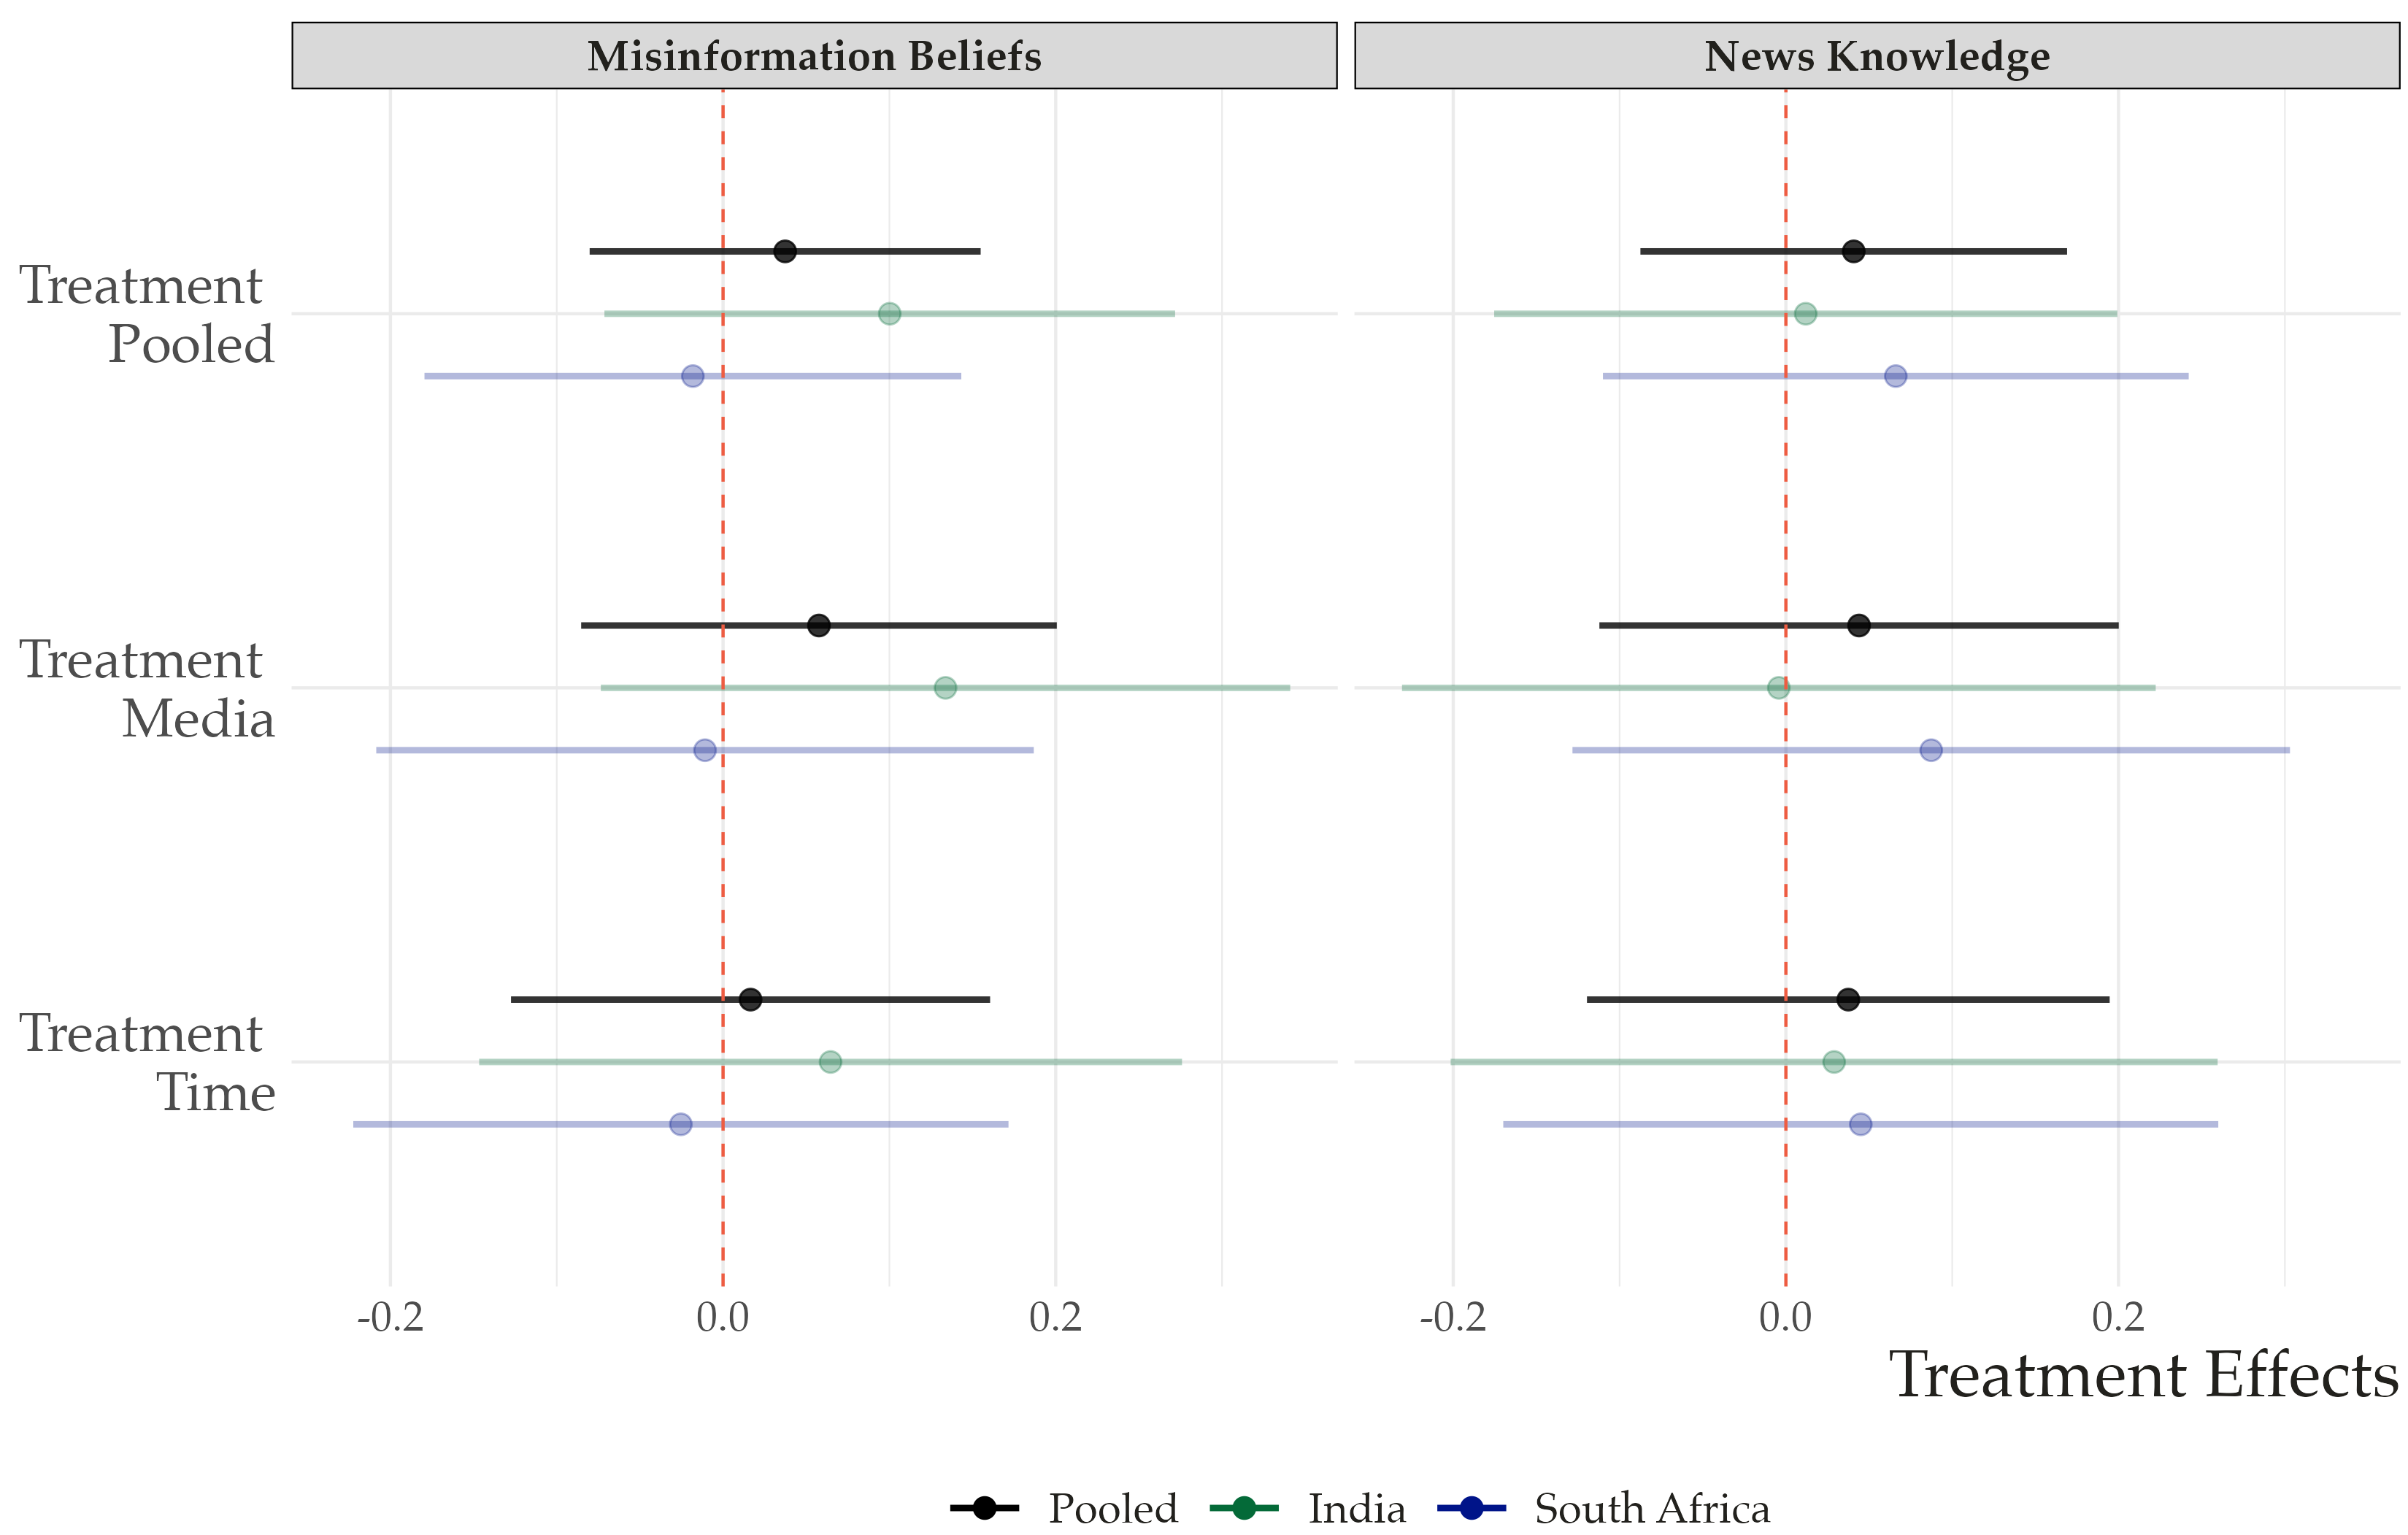
\includegraphics[scale=.37]{h2_itt}
\end{center}

\end{frame}


\begin{frame}{Polarization} \small  

Would a potential reduction in exposure to misinformation, hate speech, and incivility reduce
\begin{enumerate}
\item partisan animosity?
\item ethnic/racial prejudice?
\end{enumerate}

\pause
\vspace{.6cm}
Series of outcomes related to ingroup and outgroup attitudes
	\begin{itemize}
	\item Outcomes \begin{itemize} \item overall feelings \item traits \item willingness to participate in social activities \end{itemize}
	\item Groups
	\begin{itemize}
	\item in India: BJP \& Congress voters; Hindu \& Muslim citizens
	\item in South Africa: ANC \& DA voters; Black \& White citizens
	\end{itemize}
	\end{itemize}

\end{frame}


\begin{frame}{Polarization} \small  
\begin{center}
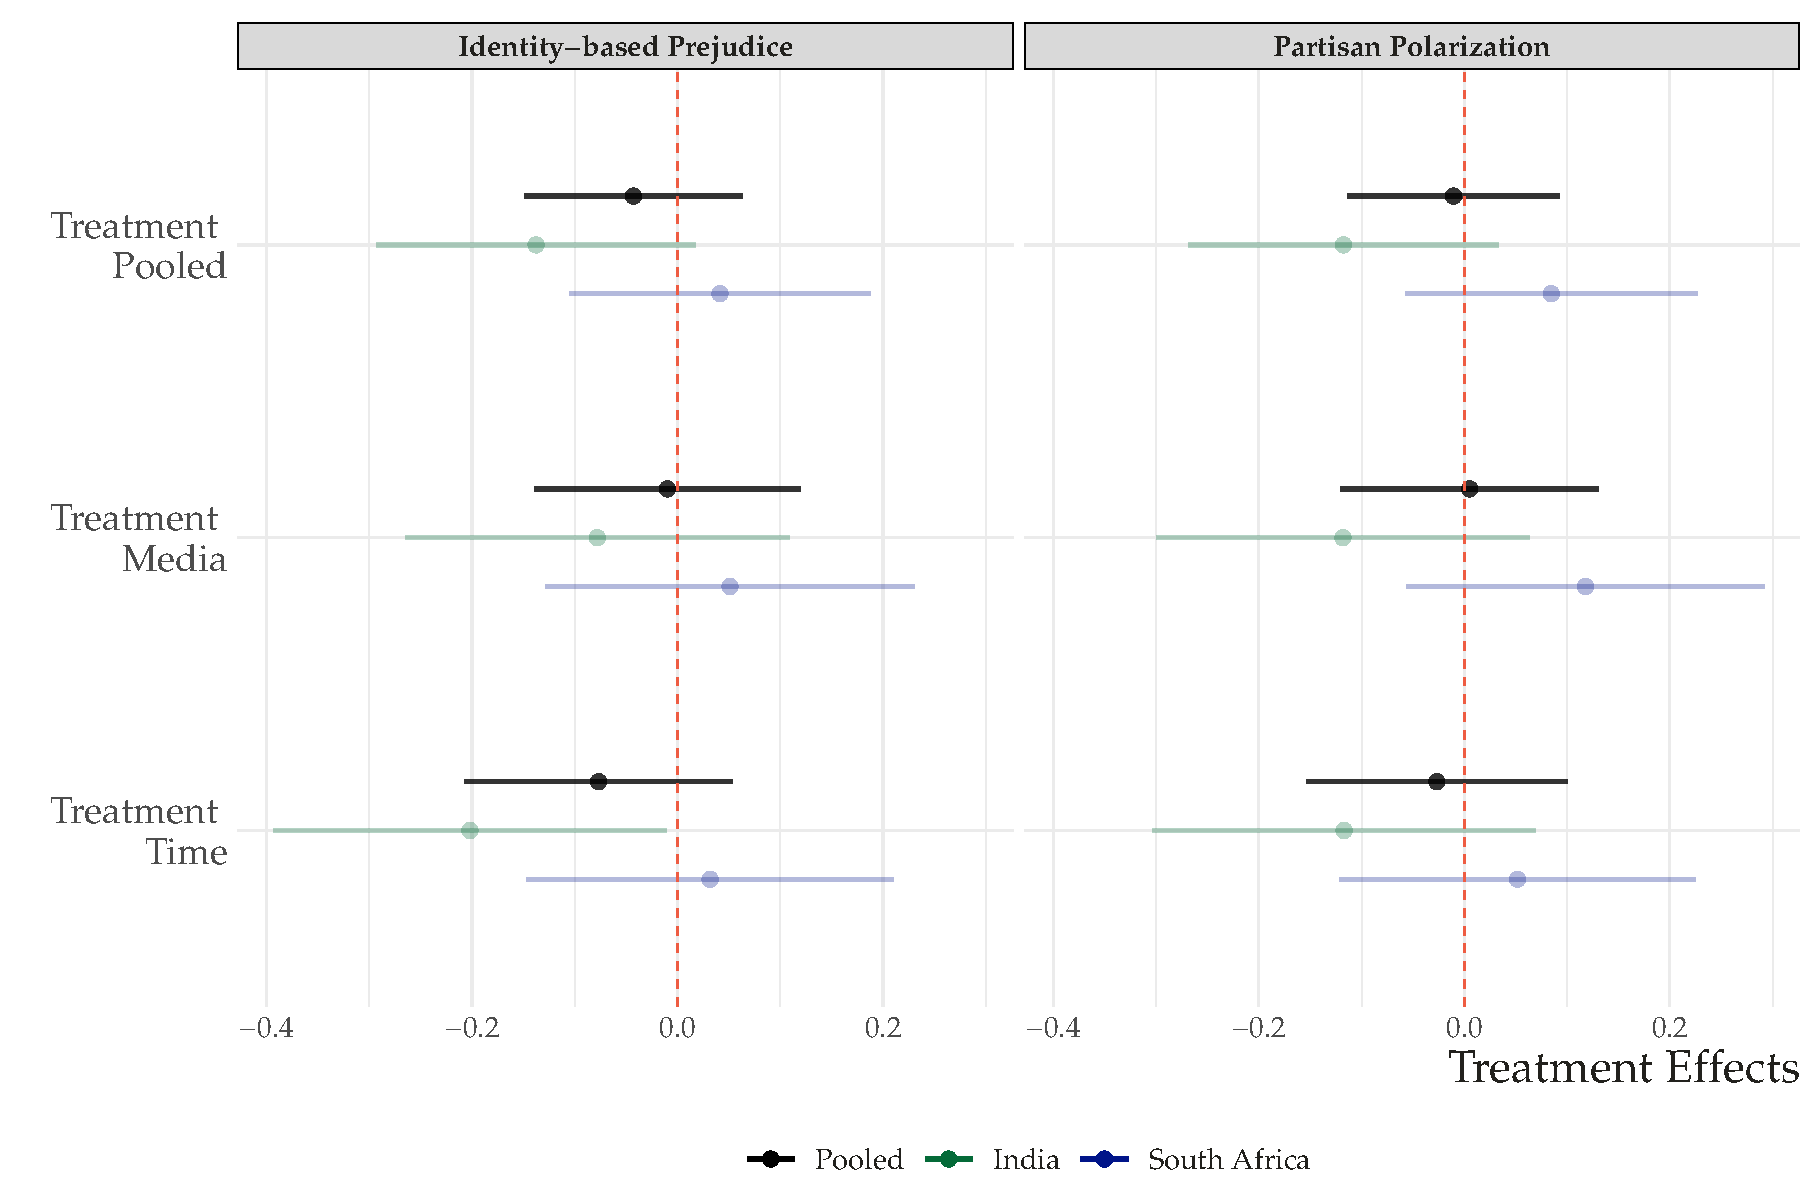
\includegraphics[scale=.37]{h_polarization}
\end{center}
\end{frame}


\section{Concluding thoughts}


\begin{frame}[plain]
\vspace{3cm}
\centering
\LARGE 
Concluding thoughts

\end{frame}


\begin{frame}{Concluding thoughts} \small  

Summary

\begin{itemize}
\item WhatsApp is an important channel through which voters receive
misinformation and news in India and South Africa
\item Reduced exposure to such information does not mechanically affect accuracy perceptions
\item Reduced exposure to such information \textit{sometimes} affects outgroup or outpartisan attitudes 
\end{itemize}

\pause 
\vspace{.25cm} 

Next steps

\begin{itemize}
\item More HTEs and secondary outcomes to understand divergences in results across countries
\item Analyze compliance data  and estimate complier effects
\item 2-week follow-up survey: effects of ``returning'' to WhatsApp?
\item Replication during local elections in Brazil: next week 
\end{itemize}

\end{frame}


\begin{frame}[plain]
\vspace{.6cm}
\centering 
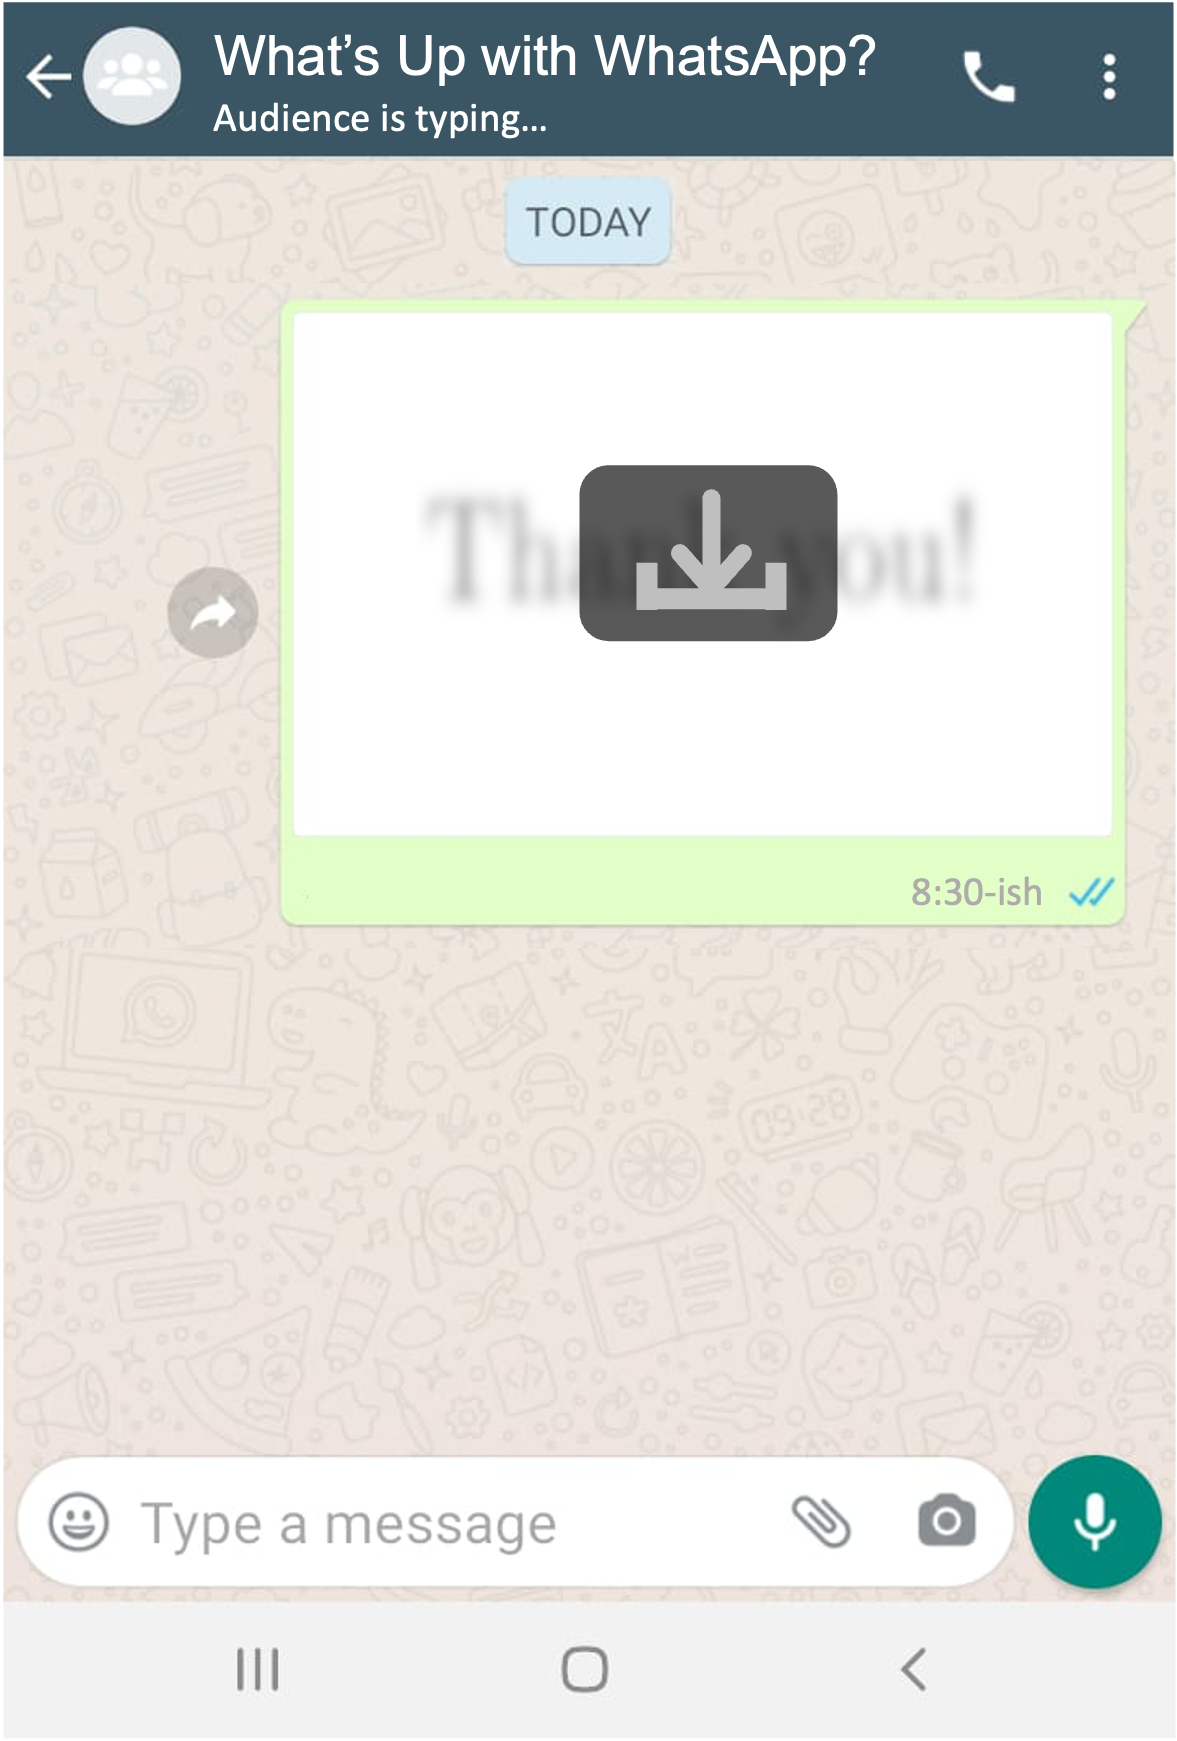
\includegraphics[scale=.6]{thanks_apsa_blur}
\end{frame}

\begin{frame}[plain]
\vspace{.6cm}
\centering 
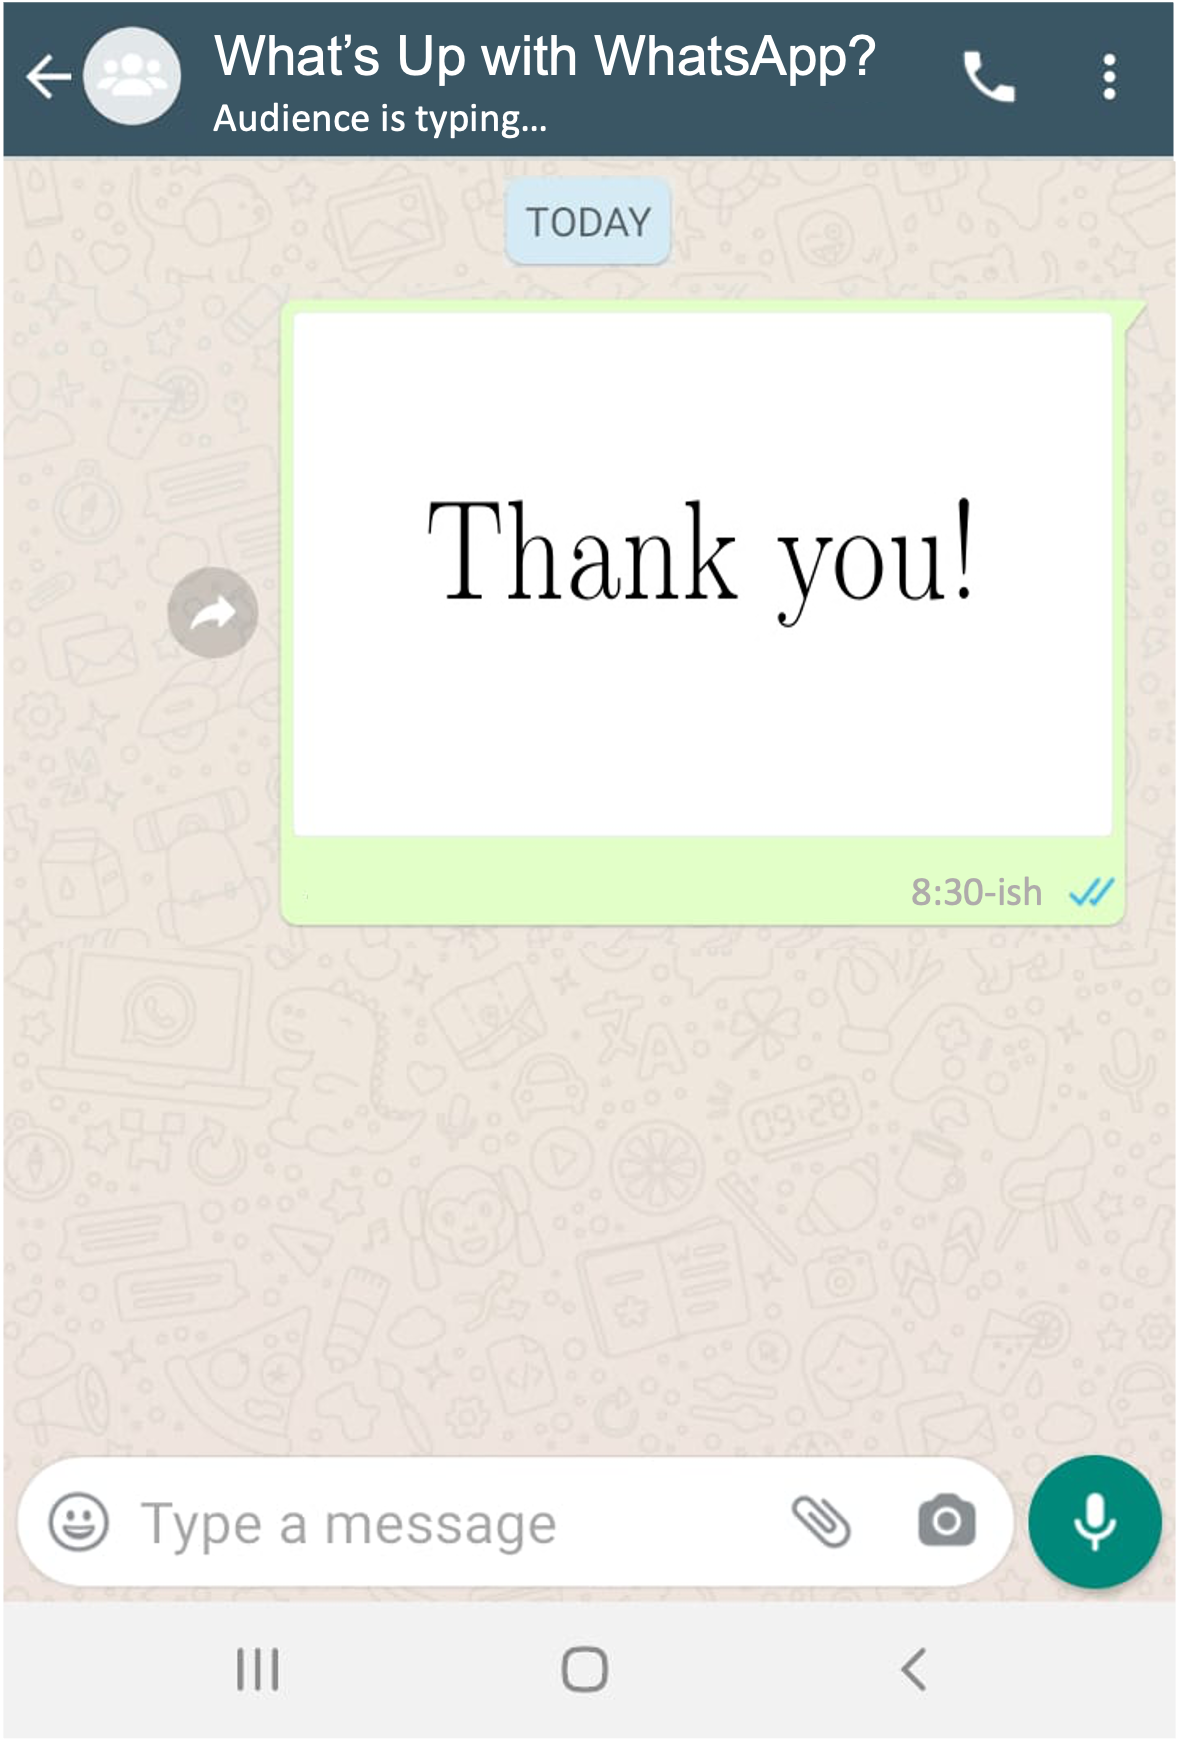
\includegraphics[scale=.6]{thanks_apsa_clear}
\end{frame}


\end{document}